\begin{figure}[ht]
\centering
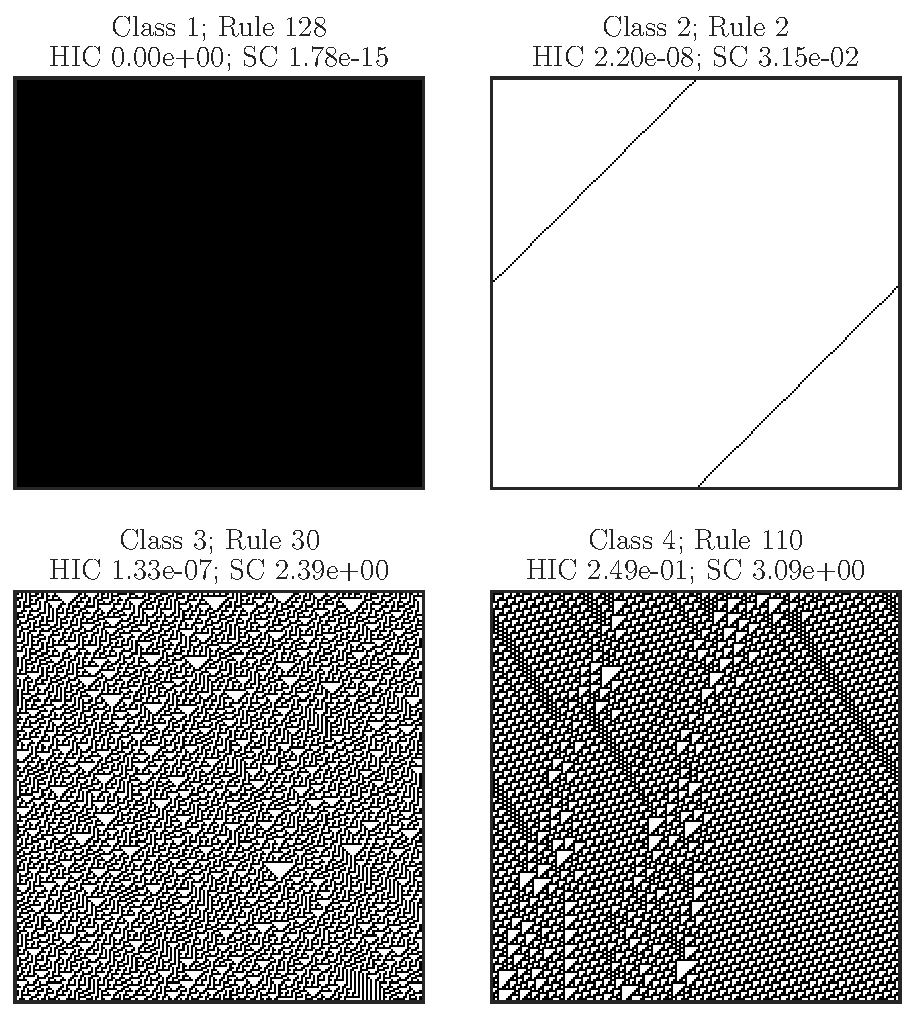
\includegraphics[width=0.7\textwidth]{figures/eca_images_and_complexity}
\caption{Example ECA rules from the four Wolfram classes. Each ECA has a state
    size of $N=200$ states and is run for $400$ steps. The latter $200$ steps
    are visualized above. We compute the HIC for each ECA using $L=3$ levels.}
\label{fig:eca_images_and_complexity}
\end{figure}

\section{Experiments}

\subsection{Experimental Setting}

We examine HIC empirically using elementary cellular automata (ECA). We also
compare HIC to statistical complexity for varioius ECA. Cells in an ECA
can take on one of two states. The update rule for a given state depends on the
state at the previous time step along with its two neighbors; hence there are
$2^{(2^3)} = 256$ possible ECAs. \citet{wolfram1983} proposed a four class
system to categorize ECA rules by their typical behavior. Class 1 ECAs converge
to a constant state, class 2 ECAs tend to exhibit periodic oscillations, class
3 ECAs display random-like behavior, and class 4 ECAs show complex behavior.
Complex behavior of an ECA is not well defined and is determined mostly through
inspection. The complex ECAs usually have various high-level structures
propagating through time with some degree of apparant randomness interspersed
between. Despite the simplicity of the rules, ECAs can yield astonishingly
complex behavior. Rule 110, for example, has been shown to be computationally
universal~\citep{cook2004universality}. We follow the Wolfram classification
given by~\citet[table 2]{martinez2013note} to classify all 256 ECA rules.

For each ECA we use a state size of $N$. The information in the initial state
requires at least $N/2$ updates to propagate accross the complete state space.
We update the ECA for $2N$ time steps and discard the first $N$ which provides
a buffer for information in the initial state to fully propagate. We use a
circular update so the cells at the edges are influenced by neighbors at the
opposite edge of the state.  Because of this, rules which propagate information
unidirectionaly can influence the full state space after $N$ updates.

We use the remaining $N \times N$ cells to compute the HIC. At each level we
set $X^\ell$ and $Y^\ell$, the variables used to compute the mutual information
in equation~\ref{eq:mutual_information}, to be neighboring sequences each
consisting of $\ell$ cells. So for the first level ($\ell = 1$) $X$ and $Y$ are
single and consecutive cells, for $\ell = 2$ the variables are consecutive but
disjoint pairs of cells, and so on. We estimate the distributions $P(X^\ell)$
and $P(X^\ell \mid Y^\ell)$ used to compute the mutual information at each
level from counts over the states.

To construct the causal states for statistical complexity, we use the
Kullback-Leibler divergence with a threshold of $1.0$. We use a past light cone
with $T_{\textrm{P}}=2$ and a future light cone with $T_{\textrm{F}} = 3$.  For
each time step the number of states in the light cone grows by two. For
example, the third time step of the future light cone contains five cells. As
with HIC we esimtate the distributions using counts over the states.

\begin{figure}[ht!]
\centering
\begin{subfigure}{\textwidth}
    \centering
    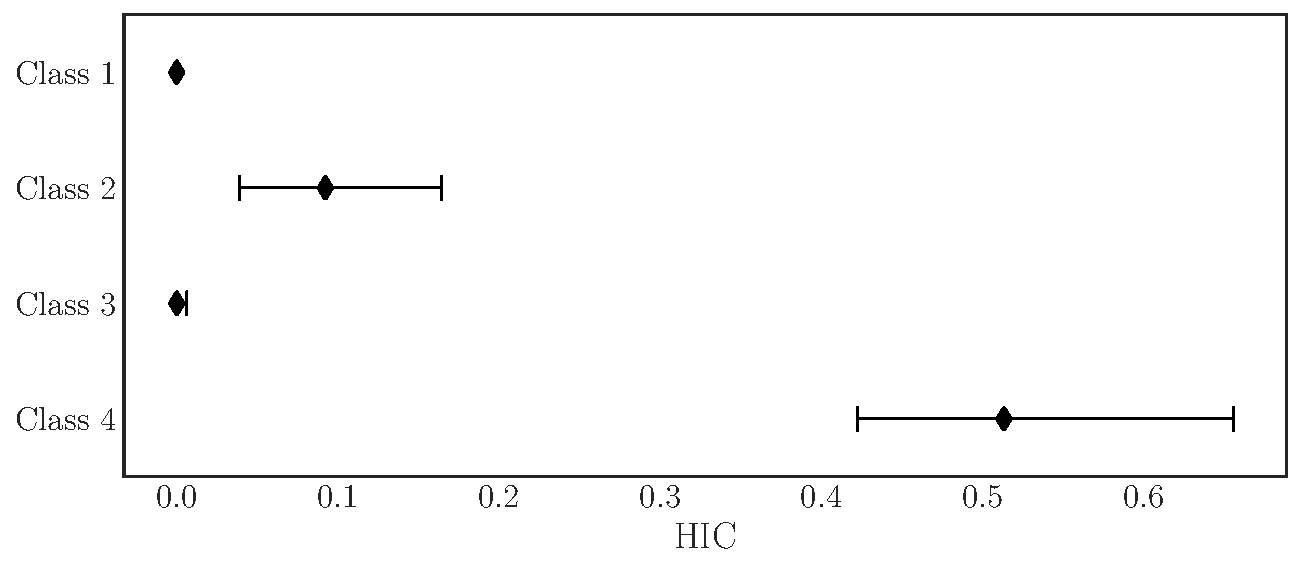
\includegraphics[width=0.8\textwidth]{figures/hic_by_class}
    \caption{Hierarchical information content (HIC)}
    \label{fig:hic_by_class}
\end{subfigure}
\begin{subfigure}{\textwidth}
    \centering
    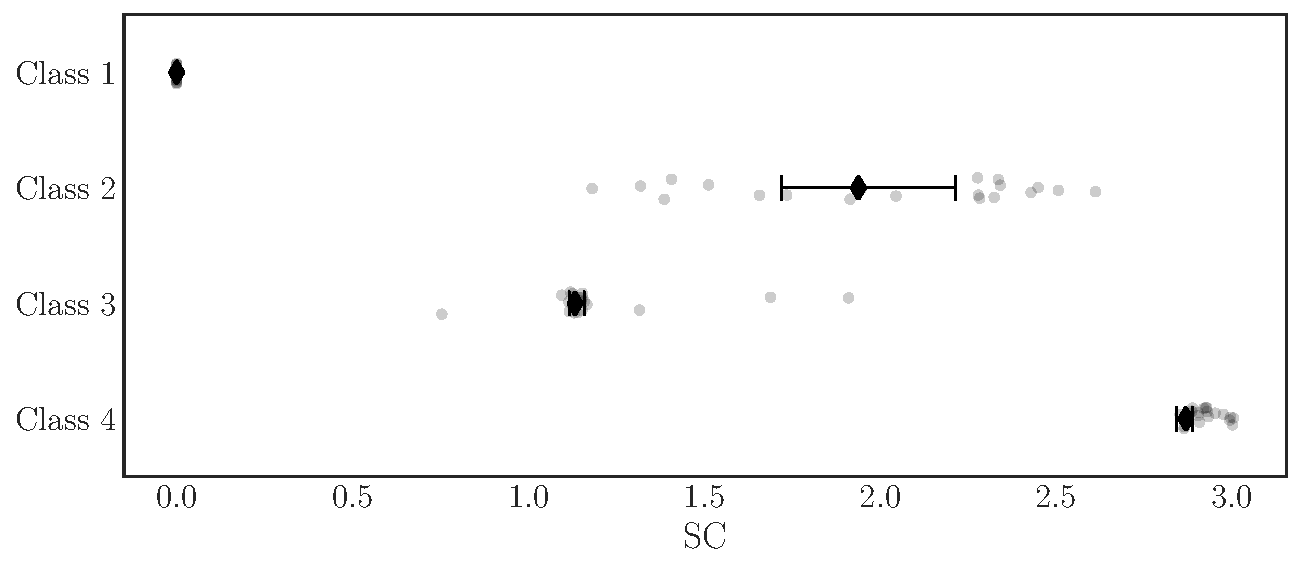
\includegraphics[width=0.8\textwidth]{figures/sc_by_class}
    \caption{Statistical complexity (SC)}
    \label{fig:sc_by_class}
\end{subfigure}
\caption{The median and 95\% confidence intervals for the HIC for each Wolfram
    class. We compute these by randomly sampling 100 rules with random initial
    states and computing the HIC of each. For each class, the first twenty
    trials within one standard deviation of the median are plotted.}
\label{fig:complexity_by_class}
\end{figure}


\subsection{Comparing HIC to Statistical Complexity}

Figure~\ref{fig:eca_images_and_complexity} shows a canonical ECA rule from each
class: rule 128 is class 1, rule 2 is class 2, rule 30 is class 3, and rule 110
is class 4. For these simulations we use $N\!=\!200$ and an initial state of all
inactive cells (zeros) with a single active cell (one) at the center. We
compute the HIC over $L\!=\!3$ levels. The HIC is given for each rule above the
corresponding image. Note that HIC correctly distinguishes rule 110 as being
the most complex ECA from the remainder, which have HICs very close to zero.
Note in particular that the HIC of the class 3 ECA (rule 30) is even smaller
than the corresponding class 2 ECA (rule 2). In this case HIC peaks inbetween
order and disorder, as desired. We also see that the statistical complexity
(SC) correctly orders the rules from each class. However, unlike HIC the class
3 ECA (rule 30) has a fairly large statistical complexity. This is the case
because the ECA exhibits randomness over the spatial dimension but has some
structure over the temporal dimensions.

Figure~\ref{fig:complexity_by_class} demonstrates that both HIC and statistical
complexity can distinguish between the four Wolfram complexity classes. These
results are obtained by sampling $100$ rules for each of the four ECA classes.
Each rule is run from a random initial state for $1000$ steps. We use a state
size of $N\!=\!500$ and hence a $500 \times 500$ grid to compute the
corresponding complexity measure. For these experiments we use $L=6$ levels for
the HIC. The class medians are well separated by the median HIC
(fig.~\ref{fig:hic_by_class}) with the 95\% confidence interval of class 4
distinct from that of any other class.

We also plot in figure~\ref{fig:hic_by_class} the first twenty trials for each
class with an HIC within one standard deviation of the median. Rules from ECA
class 2 have the widest range of HIC. Qualitative inspection of the high HIC
results shows many cases where the resulting state is simply shifted to the
left or right by the rule. The state exhibits a simple periodic pattern over
time but because of the random initialization, the pattern over space does not
appear to be simple. This is one failure mode of HIC -- it does not
capture the simplicity over the time dimension given that it is only applied to
the space dimension.

The statistical complexity medians are less well separated than those computed
from the HIC. On the other hand, the statistical complexity
(fig.~\ref{fig:sc_by_class}) has narrower 95\% confidence intervals for all
classes. Overall, both measures are quite good at distinguish complex class 4
ECA from the rest. Both measures could be useful depending on whether one
intends to measure process or structural complexity. The two may also be
combined to produce a single more comprehensive measure.

\subsection{Number of Levels}

\begin{figure}[t]
\centering
\begin{subfigure}{0.45\textwidth}
  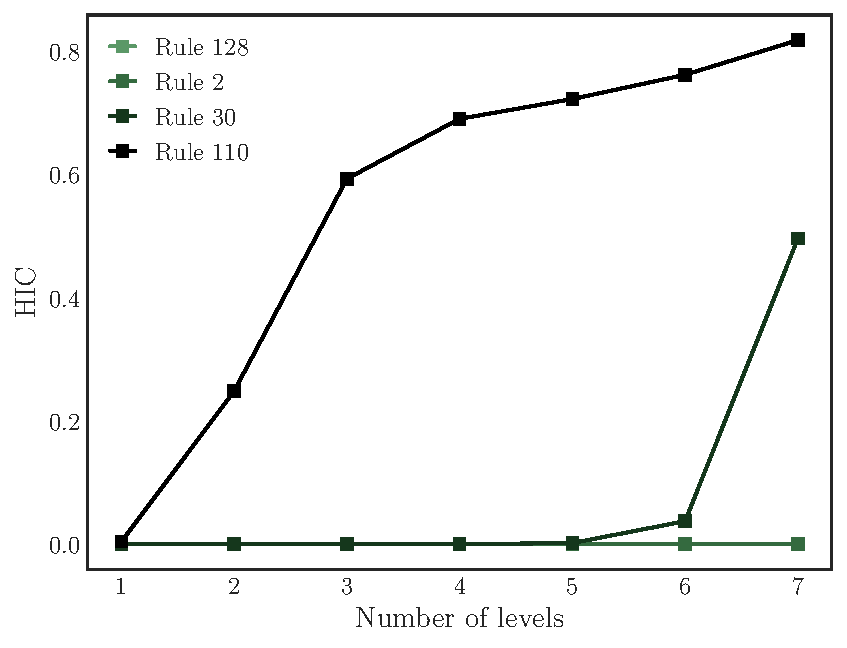
\includegraphics[width=1.0\textwidth]{figures/hic_vs_num_levels_size_200}
  \caption{State size $N = 200$}
  \label{fig:hic_levels_200}
\end{subfigure}
\begin{subfigure}{0.45\textwidth}
  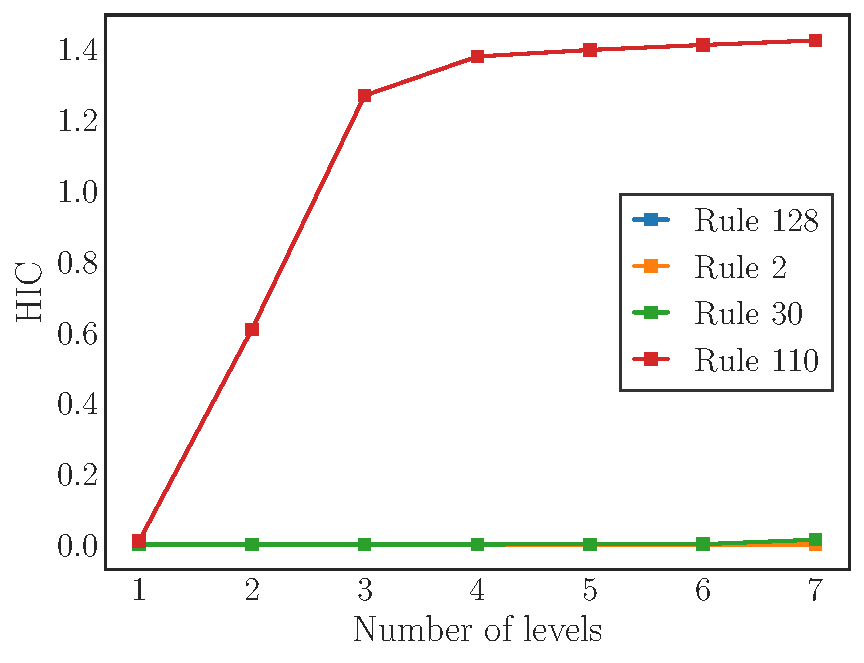
\includegraphics[width=1.0\textwidth]{figures/hic_vs_num_levels_size_500}
  \caption{State size $N = 500$}
  \label{fig:hic_levels_500}
\end{subfigure}
\caption{We show the HIC versus the number of levels $L$ used in the
    computation. We compute the HIC for one rule from each of the four Wolfram
    classes. Each ECA is run for $2N$ time steps and the HIC is computed from
    the latter half.}
\label{fig:hic_vs_levels}
\end{figure}

Using the same four rules (class 1 rule 128, class 2 rule 2, class 3 rule 30
and class 4 rule 110), we observe the effect of the number of levels on the HIC
in figure~\ref{fig:hic_vs_levels}. Figure~\ref{fig:hic_levels_200} uses a state
size of $N\!=\!200$, and figure~\ref{fig:hic_levels_500} uses a state size of
$N\!=\!500$. In both figures, we see that the class 1 and 2 rules (the curves
overlap at zero) do not grow with an increase in the number of levels. The
class 4 rule grows but plateaus with the number of levels. We expect to see a
plateau once the size of the variables $X^\ell$ and $Y^\ell$ fully capture the
the largest structures, and so the mutual information should become constant.
This shows that complexity does not grow via compositions of order from order.
Interposing disorder somewhere near the level of the largest structures would
result in further complexity growth.

The class 3 ECA is the only one which exhibits a qualitative difference between
the two figures. This is simply a finite sample statistical artifact which is
instuctive to elucidate. In the $N\!=\!200$ case, we do not have enough states to
estimate the mutual information at the highest level ($\ell\!=\!7$) accurately.
The mutual information consists of two terms, the entropy of the single
variable $H(X^\ell)$ and the conditional entropy between the two variables
$H(X^\ell \mid Y^\ell)$. The entropy requires fewer samples to estimate
accurately than the conditional entropy. For example $X^7$ can take on $2^7$
possible values whereas the pair $(X^7, Y^7)$ admits $2^{14}$ distinct values.
With insufficient sample sizes, the conditional entropy shrinks prior to the
entropy and the mutual information is artificially inflated. This can be
remedied by increasing $N$. However, a parametric or otherwise more sample
efficient model for $P(X)$ and $P(X \mid Y)$ is an alternative that will likely
scale more robustly with the number of values of $X^\ell$.
